\documentclass[11pt]{article}

\usepackage{amsmath,amssymb,amstext,amsthm, standalone}
\usepackage{geometry}
\usepackage{fancyhdr}
% \usepackage[pdftex]{graphicx}
\usepackage{xcolor}
\usepackage{tikz}
\usepackage{amssymb}

\geometry{
  verbose,
  dvips,
  width=430pt, marginparsep=0pt, marginparwidth=0pt,
  top=90pt, headheight=12pt, headsep=20pt, footskip=30pt, bottom=80pt}

\setlength{\parskip}{\medskipamount}
\setlength{\parindent}{0pt}

\linespread{1.05}

\newtheorem{theorem}{Theorem}
\newtheorem{lemma}[theorem]{Lemma}
\newtheorem{proposition}[theorem]{Proposition}
\newtheorem{corollary}[theorem]{Corollary}
\newtheorem{conjecture}[theorem]{Conjecture}
\newtheorem{obs}{Observation}
\newtheorem{clm}{Claim}
\newtheorem{ques}{Question}
\newtheorem{problem}{Problem}

\newtheorem{ex}{Example}


\newcommand{\spc}{\hspace{0.08in}}
\newcommand{\vs}{\vspace*{.1in}}
\newcommand{\E}{\mathbb{E}}
\newcommand{\Prob}{\mathbb{P}}
\newcommand{\edit}[1]{\emph{\textcolor{blue}{#1}}}


\renewenvironment{proof}{{\noindent \textbf{\textit{Proof.}}}}
{\hfill $\Box$ \vspace*{0.1in}}
\newenvironment{proofc}{{\noindent \textit{Proof of Claim.}}}
{\hfill $\Box$}


\begin{document}
\begin{huge}
    \begin{center}
        Checkpoint
    \end{center}
\end{huge}
\begin{large}\begin{center}\bf 14.5: The Chain Rule \end{center}
\end{large}

\vs\vs

\begin{problem}
Write $f(x)= \cos\left({\sqrt{5e^{-7x}}}   \right)$ as a composition of functions using different variables.
\end{problem}

\begin{problem}
If $f_x = 8xy$ and $f_y = \tan^{-1}(x+y)$ what is $\frac{dy}{dx}$?
\end{problem}

\begin{problem}
Draw the tree diagram for the following composition of functions and label the edges with partials/derivatives. $w=f_1(x,y,z)$, $x=f_2(s,t)$, $y= f_3(s)$, $z = f_4(t)$, $s = f_5(r, \theta)$, and $t = f_6(r,\theta)$.
\end{problem}


\begin{problem}
In the above problem find an expression for $\frac{\partial w}{\partial r}$.
\end{problem}




\newpage

\section{Answers}

\begin{enumerate}
    \item $y=\cos{u}$, $u= \sqrt{v}$, $v = 5e^{w}$, $w=-7x$.
    \item $-8xy/\tan^{-1}(x+y)$.
    \item 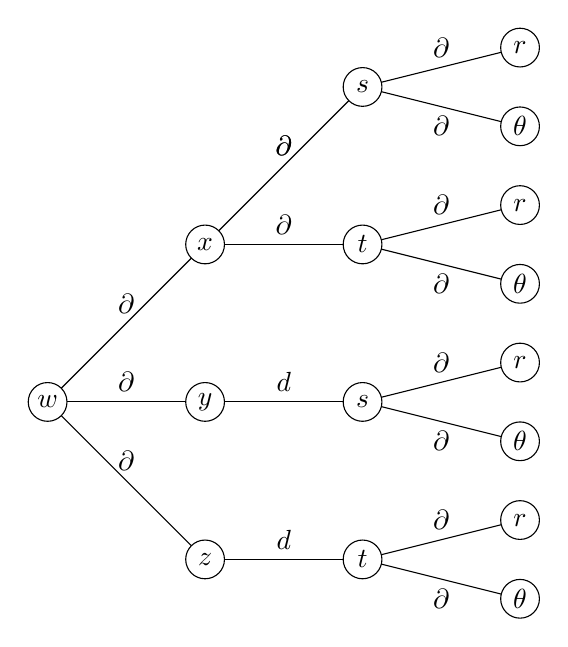
\begin{tikzpicture}
%% Graph %%

\draw (0,0) -- (2,2);
\draw (0,0) -- (2,0);
\draw (0,0) -- (2,-2);
\draw (2,2) -- (4,2);
\draw (2,2) -- (4,4);
\draw (2,0) -- (4,0);
\draw (2,-2) -- (4,-2);


\draw (4,4) -- (6,4.5);
\draw (4,4) -- (6,3.5);
\draw (4,2) -- (6,2.5);
\draw (4,2) -- (6,1.5);
\draw (4,0) -- (6,.5);
\draw (4,0) -- (6,-.5);
\draw (4,-2) -- (6,-1.5);
\draw (4,-2) -- (6,-2.5);


\draw[fill = white] (0,0) circle (7pt);

\draw[fill = white] (2,2) circle (7pt);

\draw[fill = white] (2,0) circle (7pt);

\draw[fill = white] (2,-2) circle (7pt);

\draw[fill = white] (4,4) circle (7pt);

\draw[fill = white] (4,2) circle (7pt);


\draw[fill = white] (4,0) circle (7pt);

\draw[fill = white] (4,-2) circle (7pt);



\draw[fill = white] (6,4.5) circle (7pt);

\draw[fill = white] (6,3.5) circle (7pt);

\draw[fill = white] (6,2.5) circle (7pt);

\draw[fill = white] (6,1.5) circle (7pt);

\draw[fill = white] (6,.5) circle (7pt);

\draw[fill = white] (6,-.5) circle (7pt);

\draw[fill = white] (6,-2.5) circle (7pt);
\draw[fill = white] (6,-1.5) circle (7pt);



\node at (1,1.25) {$\partial$};
\node at (1,0.25) {$\partial$};
\node at (1,-.75) {$\partial$};
\node at (3,2.25) {$\partial$};
\node at (3,3.25) {$\partial$};
\node at (5,4.5) {$\partial$};
\node at (5,3.5) {$\partial$};
\node at (3,3.25) {$\partial$};
\node at (5,2.5) {$\partial$};
\node at (5,1.5) {$\partial$};
\node at (5,0.5) {$\partial$};
\node at (5,-.5) {$\partial$};
\node at (5,-2.5) {$\partial$};
\node at (5,-1.5) {$\partial$};


\node at (3,.25) {$d$};
\node at (3,-1.75) {$d$};





\node at (0,0) {$w$};
\node at (2,2) {$x$};
\node at (2,0) {$y$};
\node at (2,-2) {$z$};
\node at (4,4) {$s$};
\node at (4,2) {$t$};
\node at (4,0) {$s$};
\node at (4,-2) {$t$};



\node at (6,4.5) {$r$};
\node at (6,3.5) {$\theta$};

\node at (6,2.5) {$r$};
\node at (6,1.5) {$\theta$};

\node at (6,.5) {$r$};
\node at (6,-.5) {$\theta$};

\node at (6,-1.5) {$r$};
\node at (6,-2.5) {$\theta$};







\end{tikzpicture}
    \item $\frac{\partial w}{\partial r} =   (\frac{\partial w}{\partial x}   )  (\frac{\partial x}{\partial s}   )  (\frac{\partial s}{\partial r}   )+   (\frac{\partial w}{\partial x}   )  (\frac{\partial x}{\partial t}   )  (\frac{\partial t}{\partial r}   ) +   (\frac{\partial w}{\partial y}   )  (\frac{dy}{ds}   )  (\frac{\partial s}{\partial r}   ) +   (\frac{\partial w}{\partial z}   )  (\frac{dz}{dt}   )  (\frac{\partial t}{\partial r}   )$
\end{enumerate}



\end{document} 